\documentclass[12pt, letterpaper]{article}
\usepackage[utf8]{inputenc}
\usepackage{amssymb}
\usepackage{graphicx}
\usepackage{enumerate}
\usepackage{enumitem}
\usepackage{mathtools}
\usepackage[linguistics]{forest}
\usepackage[ruled,linesnumbered]{algorithm2e}
\usepackage{hyperref}
\usepackage{siunitx}
\usepackage{amsmath,amssymb,amsthm}
\usepackage[utf8]{inputenc}
\usepackage[english]{babel}


\renewcommand{\baselinestretch}{1.5}
\setlength{\topmargin}{5.75cm} \setlength{\textheight}{23.5cm}
\setlength{\oddsidemargin}{0.25cm}
\setlength{\evensidemargin}{0.25cm} \setlength{\textwidth}{16.2cm}
\begin{document}
\title{\textbf{Satisfiability Test of Clauses and its Application}}
\author{Tyler Mack Johnson $\|$ Sawanth Mythrey Bhonagiri $\|$ Venkata Revanth Kollipara}
\date{November 2021}
\maketitle
\newpage
\setlength{\topmargin}{-1.75cm} \setlength{\textheight}{23.5cm}
\setlength{\oddsidemargin}{0.25cm}
\setlength{\evensidemargin}{0.25cm} \setlength{\textwidth}{16.2cm}
\section*{Objective}
To encode the n-queens problem into propositional logic, we need to write a program to generate a DIMACS CNF (Conjunctive Normal Form) encoding of the problem. The generated file can then be passed to a SAT solver such as MiniSat.
\section*{Software Required/Used}
Linux Operating System, Visual Studio Code, MiniSat
\section*{Report}
\begin{itemize}
    \item The problem is to consider n number of rows and columns such that no two queens should be on the same row, column or diagonal and there should be at least one queen at any given row or column
    \item First, in our Linux Operating System, we downloaded MiniSat
    \item Next, we wrote a program using Python programming language to generate the DIMACS CNF encoding of the n-queen problem
\end{itemize}
The algorithm for the python script is explained below.\\
\textbf{\underline{Step 1:}} Set a variable $n$ to be the number of queens (as well as rows and columns) \\
\textbf{\underline{Step 2:}} For each i (row) we append to the DIMACS CNF file a line with the clause $P_{i,0} \vee{} P_{i,1} \vee{} ... \vee ... P_{i,n} $. This assures that there must be one queen in each row of the board\\
\textbf{\underline{Step 3:}}
Now, the queens should not be repeated in the same columns
\begin{itemize}
    \item	Loop through every column in the same row and disallow two queens to exist with $\lnot{} P_{i,j} \wedge{} \lnot{} P_{i,j2}$ where $j2 = 0 \rightarrow{} n$ and $j2 \neq{} j$
\end{itemize}
\textbf{\underline{Step 4:}}
Also, make sure that there is no queen repeated in the same row
\begin{itemize}
    \item	Loop through every column in the same row and disallow two queens to exist with $\lnot{} P_{i,j} \wedge{} \lnot{} P_{i2,j}$ where $i2 = 0 \rightarrow{} n$ and $i2 \neq{} i$
\end{itemize}
\textbf{\underline{Step 5:}}
Now there shouldn't be any queens in any same diagonal
\begin{itemize}
    \item Loop through each diagonal $i2,j2$ pair (centered around each position $i,j$) while $i2 \in{} 0 \rightarrow{} n$ and $j2 \in{} 0 \rightarrow{} n$
\end{itemize}
\textbf{\underline{Step 6:}}
After all the above conditions satisfy, write all of them into a file and save as out.sat
\begin{itemize}
    \item After the code started working, we wrote this all out to a file and saved as out.sat, and checked its satisfiability, using MiniSat
\end{itemize}
\textbf{\underline{Note:}}
\begin{itemize}
    \item We encode each $P_{i,j}$ as $i + (j * n) + 1$ so that we can use the variables $1 \rightarrow{} n$ inclusive
    \item Additionally, we keep track of how many clauses are appended so that the file can be began with \texttt{p cnf <number of variables ($n^2$)> <number of clauses>}
\end{itemize}


\section*{Results}
\begin{itemize}
    \item For $n=4$, the result is:\\
    \texttt{-1 -2 \textbf{\textit{3}} -4 \textbf{\textit{5}} -6 -7 -8 -9 -10 -11 \textbf{\textit{12}} -13 \textbf{\textit{14}} -15 -16}
    \item The positions 3, 5, 12, 14 has a queen on a 4x4 board (represented below)
    \item The following figure represents the positions in which the queens present when $n=4$\\
\end{itemize}

\begin{center}
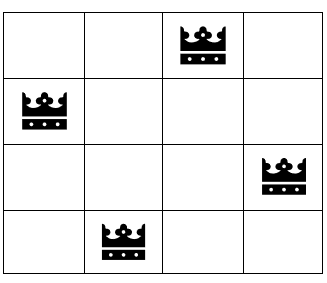
\includegraphics[scale=0.75]{image.png}
\end{center}

\end{document}
